%----------------------------------------------------------------------------------
% Exemplo do uso da classe tcc.cls. Veja o arquivo .cls
% para mais detalhes e instruções.
%----------------------------------------------------------------------------------

% Seleção de idioma da monografia. Por enquanto as únicas opções
% suportadas são 'portuguese' e 'english'
% Para impressão em frente e verso, use a opção 'twoside'. Da
% mesma forma, use 'oneside' para impressão em um lado apenas.
\documentclass[portuguese,oneside]{tcc}

%----------------------------------------------------------------
% Coloque seus pacotes abaixo.
%
% Obs.: muitos pacotes de uso comum do LaTeX, como amsmath,
% geometry e url já são automaticamente incluídos pela classe
% (veja o arquivo .cls). Isso torna obrigatória a presença destes
% no sistema para o uso desta classe, mas ao mesmo tempo o uso se
% torna mais simples.  Recomendo a instalação da versão mais
% recente da distribuição TeXLive (para Windows e UNIXes):
% www.tug.org/texlive/
%
% Pacotes e opções já incluídas automaticamente:
%
% \RequirePackage[T1]{fontenc}[2005/09/27]
% \RequirePackage[utf8x]{inputenc}[2008/03/30]
% \RequirePackage[english,brazil]{babel}[2008/07/06]
% \RequirePackage[a4paper]{geometry}[2010/09/12]
% \RequirePackage{textcomp}[2005/09/27]
% \RequirePackage{lmodern}[2009/10/30]
% \RequirePackage{indentfirst}[1995/11/23]
% \RequirePackage{setspace}[2000/12/01]
% \RequirePackage{textcase}[2004/10/07]
% \RequirePackage{float}[2001/11/08]
% \RequirePackage{amsmath}[2000/07/18]
% \RequirePackage{amssymb}[2009/06/22]
% \RequirePackage{amsfonts}[2009/06/22]
% \RequirePackage{url}
% \RequirePackage[table]{xcolor}[2007/01/21]
%----------------------------------------------------------------
% Para inserção de figuras.
\usepackage{graphicx}
% Utilize a opção 'pdftex' se você estiver usando o pdflatex (que
% permite figuras em formatos como .jpg ou .png)
%\usepackage[pdftex]{graphicx}

% Para tabelas com elementos ocupando mais de uma linha
\usepackage{multirow}
% Para frações na mesma linha (ex. ⅓).
\usepackage{nicefrac}
% Para inserir figuras lado a lado.
% \usepackage{subfigure}
% Para formatar algoritmos.
% A opção [algo2e] é necessária para evitar conflitos
% com as definições da classe.
%\usepackage[algo2e]{algorithm2e}
\usepackage{algorithmic}
% Um float do tipo algoritmo. No momento
% este pacote é incompatível com a classe.
%\usepackage{algorithm}

%----------------------------------------------------------------
% Autor (OBRIGATÓRIO)
%----------------------------------------------------------------
\author{Bruno Paz e Gabriel Rubin}

%----------------------------------------------------------------
% Título (OBRIGATÓRIO). Devem ser passados DOIS parâmetros,
% o título em português E o inglês, não importando o idioma
% escolhido. Os títulos são utilizados para a montagem da capa,
% resumo e abstract mais tarde.
%----------------------------------------------------------------
\title{Uma IA para o jogo Colonizadores de Catan}
      {An AI for the game Settlers of Catan}

%----------------------------------------------------------------
% Opções para o tipo de trabalho (OBRIGATÓRIO)
%----------------------------------------------------------------
\tipotrabalho{\ptci}         % Proposta de Trabalho de Conclusão
%\tipotrabalho{\tci}         % Trabalho de Conclusão I
%\tipotrabalho{\tcii}        % Trabalho de Conclusão II

%----------------------------------------------------------------
% Seleção do curso ("este trabalho é um requisito parcial para
% obtenção do grau de (mestre ou doutor) em Ciência da Computação").
%----------------------------------------------------------------
\curso{\cc} % Ciência da Computação
%\curso{\si} % Sistemas de Informação
%\curso{\es} % Engenharia de Software

%----------------------------------------------------------------
% Orientador (e Co-orientador, caso haja um). É OBRIGATÓRIO
% informar pelo menos o orientador.
%----------------------------------------------------------------
\orientador{Felipe Meneguzzi}
%\coorientador{Ciclano de Farias}

%----------------------------------------------------------------
% A capa é inserida automaticamente. Por isso não é necessário
% chamar \maketitle
%----------------------------------------------------------------
\begin{document}

\listofacronyms

\tableofcontents

%----------------------------------------------------------------
% Listas e sumário, nessa ordem. Somente o sumário é obrigatório,
% portanto, comente as outras listas, caso sejam desnecessárias.
%----------------------------------------------------------------
%\listoffigures       % Lista de figuras      (OPCIONAL)
%\listoftables        % Lista de tabelas      (OPCIONAL)
%\listofalgorithms    % Lista de algoritmos   (OPCIONAL)
%\listofacronyms      % Lista de siglas       (OPCIONAL)
%\listofabbreviations % Lista de abreviaturas (OPCIONAL)
%\listofsymbols       % Lista de símbolos     (OPCIONAL)
%\tableofcontents     % Sumário               (OBRIGATÓRIO)

%----------------------------------------------------------------
% Aqui começa o desenvolvimento do trabalho. Para uma melhor
% organização do documento, separe-o em arquivos,
% um para cada capítulo. Para isso, utilize o comando \include,
% como mostrado abaixo.
%----------------------------------------------------------------

%----------------------------------------------------------------------------------
% Exemplo do uso da classe tcc.cls. Veja o arquivo .cls
% para mais detalhes e instruções.
%----------------------------------------------------------------------------------

%INTRODUCAO
%----------------------------------------------------------------------------------

\graphicspath{ {TCC/} }

\frenchspacing

% ABSTRACT -----------------------------------------

%\begin{center}
%    \Large
%    \vspace{0.9cm}
%    \textbf{\textit{Abstract}}
%\end{center}

\begin{abstract}

Colonizadores de Catan é um dos principais representantes dos jogos estratégicos modernos e tem muitas características que o tornam difícil de ser jogado por uma IA. Este jogo possui poucas implementações de IA disponíveis, as quais não representam desafio para um jogador. Neste trabalho, propomos pesquisar algoritmos de jogo para projetar uma nova IA capaz de jogar Catan com uma boa performance contra outros agentes e humanos.

\end{abstract}

% ABSTRACT -----------------------------------------

\chapter{\label{chap:intro}Introdução}
% Comando para inserir siglas. Tanto as siglas quanto as
% abreviaturas devem aparecer em ordem ALFABÉTICA nas listas
% correspondentes. Como a classe no momento não é capaz de ordenar
% as entradas automaticamente, existem duas alternativas:
%
%    a- Insira todas as siglas e abreviaturas no começo do texto,
%    manualmente e em ordem alfabética.
%
%    b- Caso esteja em um ambiente UNIX (Linux, Mac ou Cygwin/similares),
%    utilize o script sort.sh e o makefile que acompanham a
%    classe. O makefile automaticamente compila a monografia para
%    PDF (mas assume que o latex está acessível pela linha de
%    comando). Neste caso a ordenação é feita de forma automática.
%

%Jogos de tabuleiro representam um desafio para a comunidade de Inteligência Artificial e seu estudo é importante para o desenvolvimento da área. Comumente são estudados uma classe de jogos chamados Jogos Combinatórios, como o Xadrez, Tic Tac Toe e Go. Diversas características desta modalidade faz com que ela seja menos complexa do que outras classes que são menos estudadas. Por conta disso, diversos jogos interessantes não foram explorados a fundo pela comunidade científica, embora seu estudo possa ser muito importante para o futuro da área.

Jogos de tabuleiro representam um desafio para a comunidade de Inteligência Artificial. O estudo de jogos clássicos de dois jogadores e informação perfeita, como Xadrez, Damas e Go, foram importantes para o desenvolvimento da área~\cite{MONTECARLOCATAN01}. Muitas técnicas de IA foram desenvolvidas para melhorar a performance de uma IA nestes jogos clássicos, como Minimax e \textit{Alpha-beta Pruning} ~\cite{MINIAXCHESS}. Apesar de lidar bem com jogos tradicionais, estas técnicas muitas vezes não são satisfatórias para jogos estratégicos modernos, comumente chamados de "eurogames", devido à maior complexidade de grande parte destes jogos quando comparada a jogos de tabuleiro tradicionais~\cite{MONTECARLOCATAN01}. Técnicas recentemente desenvolvidas para jogar jogos complexos, como Monte-Carlo \textit{Tree Search}, que melhorou expressivamente a performance de uma IA no clássico jogo Chinês Go ~\cite{MONTECARLOGO}, trazem novas possibilidades de progresso no desenvolvimento de técnicas voltadas para jogos estratégicos modernos~\cite{MONTECARLOFRAMEWORK}.

A categoria de jogos estratégicos modernos é de grande interesse para a comunidade de IA devido as características que estes jogos dividem com jogos de tabuleiro clássicos e jogos de videogame~\cite{MONTECARLOFRAMEWORK}. Colonizadores de Catan representa bem o arquétipo de um "eurogame", e apesar de várias implementações de IAs para este jogo existirem, nenhuma delas representa um desafio para um jogador experiente ~\cite{MONTECARLOFRAMEWORK}. Neste trabalho, pretendemos estudar como melhorar a performance de uma inteligência artificial neste jogo com o estudo das técnicas de IA para jogos de tabuleiro clássicas, como Minimax, e modernas, como Monte-Carlo \textit{Tree Search}, e então desenvolver uma solução capaz de competir com jogadores experientes e vencer outras soluções existentes.

%Colonizadores de Catan é um destes jogos que foram pouco explorados devido à sua complexidade frente aos Jogos Combinatórios. O jogo possui vários aspectos desafiadores e interessantes que fazem dele um ótimo cenário de estudo para abordar diversos problemas ainda não resolvidos pela Inteligência Artificial. Por conta disso, muitas das soluções que existem atualmente para este jogo não conseguem desafiar um jogador humano experiente.

%Avanços recentes obtidos no estudo do jogo Go trouxeram nova esperança para o estudo de jogos desafiadores como o Catan e pretendemos estudar maneiras de melhorar a performance de uma inteligência artificial nesse jogo com o estudo de algumas destas técnicas.

\sigla{IA}{Inteligência Artificial}
\sigla{IBM}{\textit{International Business Machines}}
\sigla{MDP}{\textit{Markov Decision Process}}
\sigla{MCTS}{\textit{Monte-Carlo Tree Search}}
\sigla{POMDP}{\textit{Partially Observable Markov Decision Processes}}


%----------------------------------------------------------------------------------


%REVISAO BIBLIOGRAFICA
%----------------------------------------------------------------------------------

\chapter{\label{chap:revbiblio}Revisão Bibliográfica}

%lorem ipsum dolor sit amet Capítulo~\ref{chap:intro} consetetur
%sadipscing elitr sed diam nonumy eirmod tempor invidunt ut labore
%et dolore magna aliquyam erat sed diam voluptua at vero eos et
%accusam et justo duo dolores et ea rebum stet clita kasd gubergren
%no sea takimata sanctus est lorem ipsum dolor sit amet lorem ipsum
%dolor sit amet consetetur sadipscing elitr sed diam nonumy eirmod.~\cite{PICCOLIAPL11}

%-----------------------------------------------------------------
\section{\label{sec:secao1}Jogos de Tabuleiro}

Jogos de tabuleiro oferecem um cenário de competição abstrata, onde dois ou mais jogadores competem para atingir um certo objetivo, permitindo avaliar a aptidão dos jogadores envolvidos para resolver problemas abstratos. Esta modalidade de jogos é objeto de estudo de diversas áreas do conhecimento, e é muito importante para a IA.

\subsection{\label{sec:secao1.1}IA e Jogos de Tabuleiro}

Jogos de tabuleiro são um dos temas mais antigos a serem estudados pela comunidade de Inteligência Artificial, contribuindo muito para o desenvolvimento da área. Em 1950, logo após computadores serem programáveis, um programa de Xadrez foi programado por Claude Shannon ~\cite{CLAUDESHANNONCHESS}. A razão da popularidade desse tema, é que ele pode ser representado mais facilmente do que cenários não abstratos da vida real e permitem que agentes programados testem as suas habilidades contra seres humanos, avaliando assim o progresso científico atingido pela área da Inteligência Artificial.
 
 Outra qualidade deste tema para IA, é o seu apelo ao público geral. Avanços atingidos em jogos populares, como o Xadrez, tiveram grande atenção na mídia, gerando entusiasmo em relação ao futuro da Inteligência Artificial. Episódios notórios como a vitória do \textit{DeepBlue} da IBM contra o então campeão de Xadrez, Garry Kasparov, em 1996 ~\cite{DEEPBLUEIBM}, e mais recentemente, a vitória do \textit{DeepMind} do Google contra o campeão mundial de Go ~\cite{DEEPMINDGO}, são tidos como conquistas da Inteligência Artificial que marcaram a história. Acreditamos que por conta disso, este é um objeto de estudo expressivo e relevante para a comunidade.
 
%bullet - que pode ser representado facilmente, fazendo deles ótimos ambientes para o desenvolvimento de agentes competitivos.

%bullet - Por conta disso, é um dos temas mais antigos dentro da área de inteligência artificial, contribuindo muito para o seu desenvolvimento.

%bullet - Grandes feitos dentro deste tema impulsionaram a popularidade da área, como a vitória do DeepBlue da IBM contra Kasparov, o então campeão mundial de xadrez, e a recente vitória do DeepMind do Google contra o campeão mundial de Go.

%bullet - Acreditamos assim que este é um bom objeto de pesquisa para o nosso trabalho.

\subsection{\label{sec:secao1.2}Teoria de Jogos}

Teoria de Jogos ~\cite{GAMETHEORYPRIMER} é um ramo da matemática aplicada que estuda formalmente o cenário de conflito e cooperação entre agentes racionais, e também formaliza diversos aspectos de jogos como: Estratégias, tomadas de decisão e a representação formal de um jogo, servindo como base para a pesquisa deste tema no ramo da Inteligência Artificial. Iremos abordar aqui algumas das teorias básicas que serão importantes em nosso trabalho.

A Teoria de Jogos define que jogos podem ser divididos em diversas categorias de acordo com suas características ~\cite{ARTIFICIALINTELLIGENCE4GAMES_TYPESOFGAMES}, o que ajuda a classificá-los e determinar a complexidade no desenvolvimento de um agente capaz de jogá-los, seguem algumas das classificações que serão importantes para o nosso trabalho.

Jogos são determinísticos quando não possuem nenhum elemento de chance dentro de suas regras, como o rolar de dados para a definição de alguma ação. Jogos que possuem tais elementos são estocásticos. Jogos estocásticos são mais complexos pela dificuldade de se considerar diversos futuros possíveis para o jogo.
 
Jogos de informação perfeita são aqueles onde todas as informações do estado de jogo estão disponíveis para todos os jogadores. Jogos que possuem informações obscuras, como cartas viradas para apenas um dos jogadores, apresentam maior desafio, já que eles não podem definir com precisão o estado atual do jogo, apenas estimá-lo.

Jogos de soma-zero são aqueles onde a soma final da pontuação de todos os jogadores envolvidos é sempre zero e sempre existe um vencedor. O ganho obtido por um jogador se traduz em perda para os outros jogadores e sempre é possível medir com precisão qual dos jogadores está ganhando.

O número de jogadores também influência na complexidade de um jogo. Quanto maior o número de jogadores, maior será a árvore de jogo, já que ela deve representar estados e ações para cada jogador, o que aumenta a complexidade do problema.

%\begin{itemize}
%\item Jogos são determinísticos quando não possuem nenhum elemento de chance dentro de suas regras, como o rolar de dados para a definição de alguma ação. Jogos que possuem tais elementos são estocásticos. Jogos estocásticos são mais complexos pela dificuldade de prever o resultado de uma jogada.

%\item Jogos de informação perfeita são aqueles onde todas as informações do estado de jogo estão disponíveis para todos os jogadores. Jogos que possuem informações obscuras, como cartas viradas para apenas um dos jogadores, apresentam maior desafio, já que eles não podem definir com precisão o estado atual do jogo, apenas estimá-lo.

%\item Jogos de soma-zero são aqueles onde a soma final da pontuação de todos os jogadores envolvidos é sempre zero e sempre é possível medir com precisão qual dos jogadores está ganhando e o quão próximo da vitória este jogador está.

%\item O número de jogadores também influência na complexidade de um jogo. Quando um jogo possui dois jogadores jogando competitivamente, cada jogador busca maximizar os seus pontos e minimizar os pontos do adversário. O mesmo não pode ser dito a respeito de jogos com mais de dois jogadores, onde podem existir alianças entre jogadores e o agente deve estar preparado para este tipo de comportamento.
%\end{itemize}

Estas categorias nos ajudam a avaliar os jogos de tabuleiro e considerar quais são as melhores técnicas e algoritmos que podem ser utilizados para criar um agente capaz de jogá-los. Espera-se que um agente tenha um comportamento ótimo no jogo, ou seja, que faça sempre a melhor jogada possível em qualquer situação a fim de sair vitorioso.

%bullet - Jogos podem ser divididos entre diversas categorias, o que ajuda à classifica-los e determinar a sua complexidade dentro da área de inteligência artificial. As categorias são:

%BULLETS:
%\begin{itemize}

%   \item Determinismo: Jogos podem ser determinísticos ou estocásticos, onde existem elementos de chance que não dependem do jogador. 
%   \item Observáveis (ou de Informação Perfeita ou Imperfeita): Classifica se o jogo possui elementos ocultos aos jogadores ou não.
%   \item Soma-zero: Se a soma dos pontos obtidos por todos os jogadores é sempre zero ou se pode haver diferenças entre a pontuação, sobrar ou faltar pontos.
%   \item Turnos: As ações tomadas nos jogos podem ser sempre em sequencia ou acontecer simultaneamente.
%   \item Número de Jogadores.
%   \item Tempo de Jogo: Se as ações são discretas ou em tempo real.
   
%\end{itemize}
   
%bullet - Essas categorias nos ajudam à avaliar os jogos e considerar qual o melhor algoritmo para resolve-lo. %Resolver um jogo é ter o comportamento ótimo neste, o que pode significar obter a vitória ou outro tipo de recompensa específico ao qual o agente deseja dentro do jogo.

%-----------------------------------------------------------------

\section{\label{sec:secao2}Colonizadores de Catan}

Colonizadores de Catan é um jogo de tabuleiro moderno criado pelo alemão Klaus Teuber e publicado em 1995. O jogo se popularizou rapidamente e ganhou notoriedade fora da Alemanha, fazendo com que o gênero conhecido como "eurogame" fosse reconhecido em todo o mundo ~\cite{MONTECARLOCATAN01}. Uma das principais razões do sucesso de Catan é a sua jogabilidade: as regras e funcionamento do jogo foram desenvolvidas buscando o equilíbrio entre estratégia, política entre jogadores e sorte. Este equilíbrio de jogo permite que um iniciante tenha chances de competir contra outros jogadores mais experientes e se divertir com a partida. Além disso, o jogo tem profundidade estratégica suficiente para fomentar uma forte comunidade competitiva, que cresce desde o seu lançamento.

Existem diversas implementações de agentes que jogam Colonizadores de Catan disponíveis hoje. Podemos destacar 2 implementações como sendo as melhores ~\cite{MONTECARLOCATAN01}. A primeira é proprietária da Castle Hill Studios, parte da MSN Games da Microsoft. A outra é um programa \textit{open-source} desenvolvido por Robert S. Thomas em Java chamado JSettlers.~\cite{Thomas:2002:JSR:502716.502779}

%bullet - Colonizadores de Catan é um jogo de tabuleiro modero criado por Klaus Teuber e publicado em 1995.

%bullet - O jogo se popularizou rapidamente e ganhou notoriedade fora da alemanha, ajudando a impulsionar o gênero conhecido como "eurogame".

%bullet - Inteligencias artificiais desenvolvidas para este jogo até o presente momento não são competitivas em partidas contra jogadores profissionais.

\subsection{\label{sec:secao2.1}Regras e descrição de jogo}

Colonizadores de Catan possui diversas expansões, iremos descrever aqui a sua versão básica que pode ser jogada por 3 ou 4 jogadores competitivamente. O jogo possui um tabuleiro formado por hexágonos, onde cada hexágono representa um terreno que produz um tipo de recurso: a floresta produz madeira, a plantação produz trigo, a montanha produz pedra, a mina produz tijolo, o pasto produz ovelhas e o deserto não produz recurso. Existe apenas um hexágono de deserto no jogo. Estes hexágonos podem ser configurados de diversas maneiras antes do começo da partida para permitir diferentes cenários de jogo. Um número é atribuído para cada hexágono, entre 2 e 12, exceto o deserto que não produz recurso. Cada jogador possui peças de uma cor específica para diferenciá-los dentro do tabuleiro. Estas peças representam as edificações do jogador, que podem ser: Estradas, aldeias e cidades. Estas edificações podem ser colocadas na adjacência de diferentes terrenos e ficam sempre presentes no jogo após serem construídas. A Figura 2.1 ilustra uma possível configuração de tabuleiro de jogo, onde a posição e número de cada terreno já estão configuradas.

Os jogadores possuem recursos que são obtidos de acordo com os terrenos do tabuleiro e podem ser trocados entre jogadores ou com o banco de jogo. Cercando os terrenos do jogo, existe o oceano, que possibilita aos jogadores com edificações próximas usufruir de diferentes regras para troca. O jogo ainda possui 2 dados, diversas cartas que representam os recursos de um jogador e um baralho de cartas de evento que podem ser compradas e utilizadas pelos jogadores.

Colonizadores de Catan é uma corrida por pontos entre os jogadores. Aquele que obtiver 10 pontos de vitória, vence o jogo. Para obter pontos, os jogadores devem construir edificações no tabuleiro, comprar cartas de desenvolvimento ou atingir 2 objetivos de jogo. Aldeias valem 1 ponto de vitória, cidades valem 2 e existem cartas de desenvolvimento que valem 1 ponto, já os objetivos valem 3 pontos cada. Um objetivo é ser o primeiro jogador a obter 3 cartas de cavalaria e o outro é ter a maior estrada construída durante a partida.

    \begin{figure}[H]
      \centering
      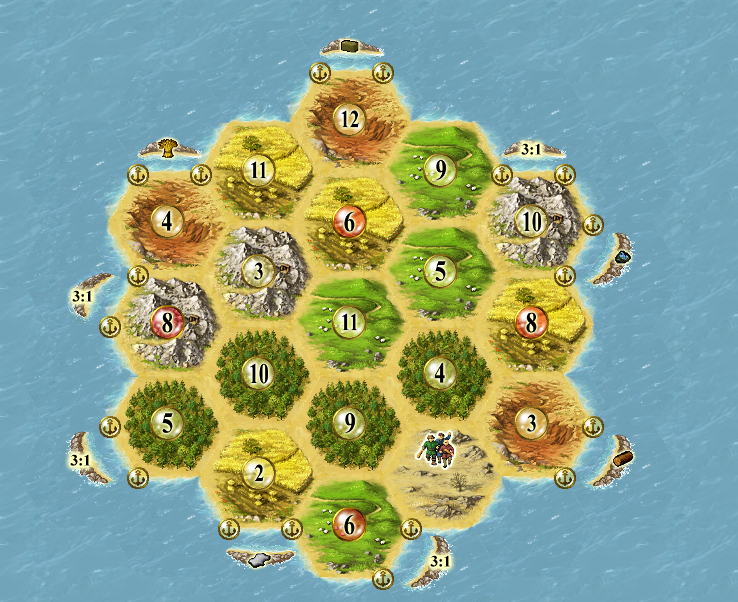
\includegraphics[width=1\textwidth]{catan.png}
      \caption{Tabuleiro do jogo}
    \end{figure}

Uma partida começa com uma configuração inicial para cada jogador dentro do tabuleiro. Na configuração para iniciantes, cada um começa com 2 aldeias e 2 estradas construídas, ou seja, 2 pontos de vitória, e algumas cartas de recurso. Os jogadores então jogam em turnos até que um deles atinja 10 pontos de vitória. No começo de seu turno, o jogador deve rolar 2 dados de 6 lados para definir quais terrenos do tabuleiro irão produzir recursos. Se o número obtido nos dados for 7, o jogador pode mover o ladrão, uma peça especial de jogo. 

O ladrão inicia a partida acima do deserto e está sempre presente no jogo. Ele pode ser visto na Figura 2.1 em sua posição inicial. Esta peça pode ser movida com o uso da carta de cavalaria por algum dos jogadores ou com os dados, como descrito anteriormente. O terreno em que o ladrão estiver não produz recursos. Isso pode ser utilizado para "negar" a produção de recursos de um jogador adversário. O jogador que mover o ladrão para um terreno que "nega" a produção de recurso de algum outro jogador, pode roubar uma carta de recurso deste jogador escolhida aleatoriamente.

Após rolar os dados, os jogadores podem então trocar recursos entre si ou com o banco de jogo. Trocas entre jogadores podem ser feitas com taxas de conversão definidas por eles mesmos, já trocas com o banco só podem ser feitas com uma taxa de 3:1, exceto se o jogador tiver uma edificação próxima ao oceano do jogo, então taxas especiais para troca com o banco se aplicam. Depois de realizar as trocas, o jogador pode então investir seus recursos para construir edificações e comprar cartas de desenvolvimento. Existem mais algumas regras específicas para a construção de edificações no tabuleiro, além de compra e uso de cartas de desenvolvimento que cada jogador deve respeitar em seu turno, mas elas não alteram este fluxo básico de jogo.

%bullet - Colonizadores de Catan, na sua versão básica, pode ser jogado por 3 ou 4 jogadores competitivamente.
%bullet - O jogo é uma corrida por pontos, o primeiro jogador que obtiver 10 pontos de vitória vence o jogo.

%bullet - Para obter pontos, jogadores devem utilizar recursos para construir edificações no tabuleiro ou comprar cartas de desenvolvimento.

%bullet - Aldeias valem 1 ponto, cidades valem 2 pontos. O jogador que tiver 3 cavalarias primeiro ganha 3 pontos, que são cartas de desenvolvimento. O jogador que tiver a maior estrada continua construida possui 3 pontos.

%bullet - Cartas de desenvolvimento são pescadas de um baralho e são consumiveis, tendo um efeito específico e imediato ou representando 1 ponto de vitória que pode ser usado no fim da partida para atingir a vitória.

%bullet - Construções são estáticas e ficam no tabuleiro até o fim da partida. Estradas permitem que o jogador expanda a sua área de atuação dentro do tabuleiro. Aldeias e cidades geram recursos para o jogador.

%bullet - O jogo possui um tabuleiro configurável com estados inciais diferentes para cada jogador.

%bullet - Jogadores podem trocar recursos entre si e com o banco do jogo.

%bullet - A cada rodada, os jogadores atiram dados para determinar qual região do tabuleiro irá produzir recursos. Jogadores com aldeias ou cidades nestas regiões ganham o recurso respectivo da região.

%bullet - O ladrão é uma peça de jogo que está sempre presente no tabuleiro. A região onde o ladrão esta colocado não produz recursos até que o ladrão saia desta região.

%bullet - Jogadores podem mover o ladrão obtendo o valor 7 nos dados ou utilizando a carta de desenvolvimento da cavalaria. Cavalaria ficam expostas em frente ao jogador para indicar quantas este possui.

\subsection{\label{sec:secao2.2}Características e desafios}

Colonizadores de Catan tem três características que o tornam complexo quando comparado aos jogos de tabuleiro clássicos ~\cite{MONTECARLOCATAN01}. Esta modalidade de jogos geralmente é determinística, observável e de 2 jogadores ~\cite{MONTECARLOFRAMEWORK}. Catan, por outro lado, é estocástico, por necessitar da rolagem de dados durante os turnos, parcialmente observável, por conter cartas de desenvolvimento que ficam abertas apenas para o jogador que as possui, e tem mais de 2 jogadores ~\cite{MONTECARLOCATAN01}.

Outro aspecto do jogo, que é bastante desafiador para agentes, é o fato de jogadores poderem trocar recursos livremente entre si, com o banco de jogo ou com um porto que estejam adjacentes. Levando em conta esse sistema de troca e a quantidade de jogadores da partida, o agente deve estar preparado para tomar decisões políticas e decidir entre fazer ou não troca de recursos com adversários ou com o banco de jogo.

%bullet - O fato de ser um jogo de vários jogadores faz com que a árvore de jogo tenha um fator de ramificação elevado.

%bullet - A rolagem de dados torna o jogo imprevisivel por ser um elemento de chance, o que torna dificil classificar a qualidade das jogadas.

%bullet - As cartas de desenvolvimento e os recursos são elementos ocultos para os outros jogadores, sendo reveladas apenas para os jogadores que as possuem.

%bullet - A troca entre jogadores também representa um desafio para uma inteligência artificial (eu sei que sim, mas ainda tenho que pesquisar mais sobre o porque).

%---------------------------------------------------------------

\section{\label{sec:secao3}Técnicas de Jogo para IA}

Esta seção apresenta algumas das técnicas de IA que são comumente aplicadas em agentes que jogam jogos de tabuleiro clássicos e servem de modelo para técnicas de IA modernas. Estudaremos estes algoritmos para modelar nosso agente que jogará Catan.

\subsection{\label{sec:secao3.1}Minimax}

 %bullet- O Minimax é um algoritmo muito utilizado como modelo para resolver jogos deterministicos, observaveis, de soma-zero, jogados em %turnos, de 2 jogadores e tempo de jogo discreto.
 
 %bullet- Esse algoritmo funciona com estados, jogadas e uma função de utilidade, para calcular quanto vale cada estado final do jogo.

 O Minimax  é um algoritmo que serve de base para grande parte dos algoritmos de busca em árvore de jogo ~\cite{GOMINIMAX}. Composto por um conjunto de estados, jogadas e uma função de utilidade, para calcular quanto vale cada estado final do jogo, sua função é encontrar a estratégia ótima, a fim de vencer a partida, construindo uma árvore de jogo que modela a competição entre dois jogadores em um jogo de soma-zero da seguinte forma:
 
\begin{itemize}

   \item De um certo estado do jogo, o algoritmo cria toda a árvore de jogo, e calcula a utilidade dos estados finais da árvore utilizando a função de utilidade. 
   \item Partindo do estado final, a utilidade de cada estado intermediário do jogo é calculado subindo pela árvore, sempre trocando entre uma etapa de maximização de utilidade e outra de minimização, para simular a jogada de ambos os jogadores, partindo do pressuposto de que ambos vão sempre buscar as jogadas ótimas, que possuem maior utilidade.
   \item Finalmente, quando a raiz é atingida, a maior utilidade é escolhida dentre os estados imediatamente abaixo do estado raiz e uma jogada é feita pela máquina.
   
\end{itemize}
    
Uma possível aplicação deste algoritmo é no jogo Tic-Tac-Toe(Jogo da Velha). Apesar de ser um jogo muito simples e com poucos recursos, a árvore gerada pelo algoritmo é de certa forma bastante profunda, visto que esta árvore representa todas a jogadas possíveis do jogador (MAX) com base nas jogadas do o oponente (MIN). Ao final da árvore, as folhas são os possíveis resultados de jogo, vitória, empate ou derrota são avaliados com um valor de utilidade, sendo a vitória de MAX o mais útil, conforme a Figura 2.2.

    \begin{figure}[H]
      \centering
      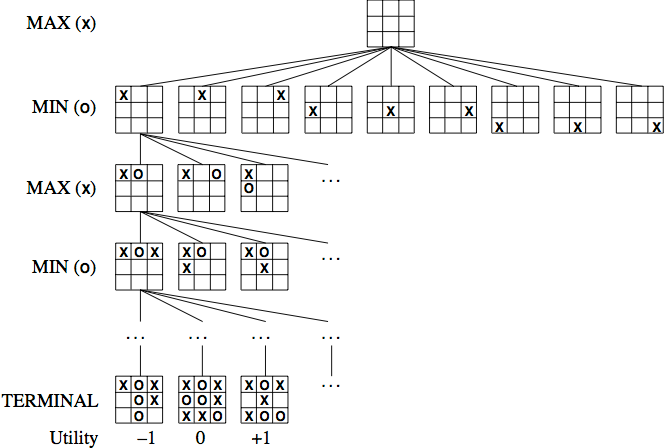
\includegraphics[width=1\textwidth]{minimax-fig1.PNG}
      \caption{Apenas uma parte da árvore gerada pelo algoritmo Minimax. Para cada ação de MIN uma nova ramificação é gerada para MAX. Ao final da árvore as folhas são o resultado do jogo, e um valor de utilidade é atribuído para cada resultado.~\cite[Cap 5, pp163-166]{AIMA}}
    \end{figure}
     
 %bullet- Este algoritmo serve de modelo ideal para resolver diversos jogos, porém é bastante custoso e complexo, devido ao seu fator de ramificação alto.%%, ou seja, a árvore de possibilidades de jogada cresce rapidamente e torna vários jogos intratáveis para um computador. 
 
 %bullet- Existem diversas maneiras de lidar com este problema, a maior parte das técnicas visam cortar a árvore de jogo afim de descartar jogadas e estados "ruins" mais rapidamente.
 
Este algoritmo serve de modelo ideal para resolver diversos jogos, porém é bastante custoso e complexo, devido ao seu fator de ramificação alto, ou seja, a árvore de possibilidades de jogadas cresce rapidamente e torna vários jogos intratáveis para um computador. Afim de evitar o crescimento da árvore gerada, algumas técnicas de corte foram elaboradas. A ideia é descartar nodos, eliminando ramificações desnecessárias, reduzindo o problema e aumentando a performance do algoritmo.
 

\subsection{\label{sec:secao3.2}Técnicas de corte para Minimax}

%\begin{itemize}
   %\item Alpha-Beta Pruning permite que estados que não seriam explorados pela regra de maximização e minimização sejam considerados durante a formação da arvore. 
   %\item Funções de Avaliação permitem que a utilidade seja calculada antes de se chegar ao fim do jogo, assim a arvore não precisa estar completa. Para avaliar jogadas não finais, o algoritmo necessita ter um conhecimento prévio das regras e estratégias do jogo e uma heurística para estimar as utilidades.
%\end{itemize}

%bullet - A desvantagem dessas abordagens é a necessidade de se ter conhecimento do domínio, as regras e a qualidade das jogadas do jogo, que é custoso e exige um estudo aprofundado do jogo, algo que muitos jogos não dispõem o que torna essas abordagens caras ou inviaveis.

%bullet - Vimos que a recompensa pode ser alcançada apenas no final do jogo, quando o agente perde ou ganha, mas isso pode ser intratavel para jogos com um grande fator de ramificação da árvore de jogo.

%bullet - Funções de evaluação permitem que se estime a possível recompensa futura de um estado baseado em conhecimento do domínio. Com isso, o Minimax não precisa necessariamente atingir um final de jogo durante a geração da árvore de jogadas.

%bullet - Tecnicas de pruning podem ser utilizadas para cortar ramos da árvore de busca sem que eles sejam visitados.

%bullet - Alpha-Beta pruning pode ser utilizado para desconsiderar as jogadas que não seriam interessantes devido à natureza do Minimax, de maximizar uma etapa e minimizar a seguinte.

%Como dito na seção anterior, um dos grandes problemas do Minimax é o tamanho da árvore de estados de jogo. Algumas técnicas visam minimizar esse problema cortando esta árvore. %que pode conter muitos estados  muitos desses estados não são úteis, ou seja, não levam a solução ótima, fazendo com que a árvore fique com um enorme número de ramificações e consequentemente bem custoso, visto que o algoritimo passa por todos os estados.Algumas técnicas visam minimizar esse problema:

\textit{Alpha-Beta Pruning} é uma técnica que pode ser utilizada para desconsiderar alguns nodos da árvore que não irão influenciar na escolha da jogada. Devido à natureza do Minimax de maximizar uma etapa e minimizar a seguinte, alguns nodos da árvore não são relevantes durante o processo de seleção e, utilizando esta técnica, podemos descartar eles mesmo antes de considerar-los como é mostrado na Figura 2.3. Conforme o caminhamento na árvore, são definidos dois valores, $\alpha$ e $\beta$:

    \begin{itemize}
    
        \item $\alpha = $ é o valor do melhor caminho já explorado até a raiz para o jogador (MAX).
        \item $\beta = $ é o valor do melhor caminho já explorado até a raiz para o oponente (MIN).
    
    \end{itemize}

    \begin{figure}[H]
      \centering
      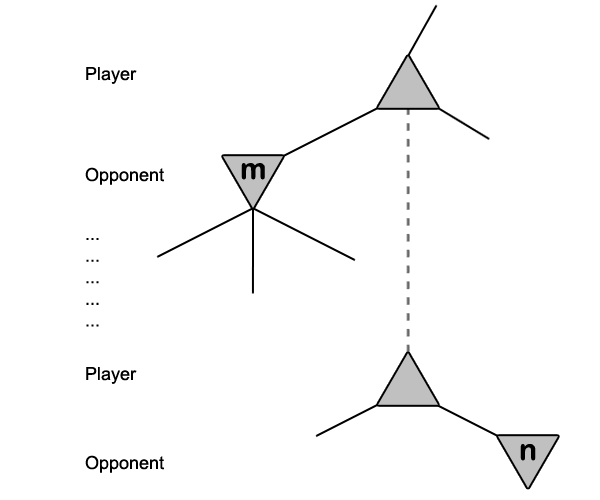
\includegraphics[width=0.6\textwidth]{pruning-fig1.png}
      \caption{A figura acima mostra um exemplo do comportamento do \textit{pruning}. Se o valor atribuído da jogada de MIN $m$ for melhor que o valor de um possível resultado de partida $n$, então a partida nunca irá resultar em $n$, por ser um resultado ruim para MAX.~\cite[Cap 5, pp167-171]{AIMA}}
    \end{figure}

Mesmo com a redução de possibilidades de jogadas que seriam ruins, a técnica \textit{Alpha-Beta Pruning} ainda precisa percorrer grande parte da árvore de jogo, o tornando não muito eficiente para jogos com uma certa complexidade. Uma solução para este problema é substituir a função de utilidade por uma Função de Estimação heurística.
Uma Função de Estimação ou \textit{Evaluation Function} tem como objetivo estimar um valor para determinado ponto do jogo, ou seja, ao invés do algoritmo percorrer todo caminho até um nodo final, ele simplesmente pode parar no meio do caminho e estimar um valor com base no que já foi percorrido. Este valor é estimado melhor quando há uma possível chance de vitória.~\cite[Cap 5, pp171-175]{AIMA}

\subsection{\label{sec:secao3.3}Expectimax}

A técnica \textit{Alpha-Beta Pruning} reduz visitas em nodos, mas ainda assim percorre grande parte da árvore de jogo. Uma forma de otimizar esta técnica é usar uma \textit{Evaluation Function}, assim o caminho percorrido será muito menor, visto que ao chegar em um certo nodo, não terminal, será estimado um valor para o mesmo, e com base nos nodos percorridos anteriormente, assumir que este nodo é terminal.

Jogos como o Catan apresentam elementos de chance, ainda não considerados nas técnicas vistas acima. O algoritmo Expectimax lida com este problema, introduzindo uma nova etapa, de nodos de chance na árvore de jogo, como mostra a figura 2.4, além dos nodos de Mínimo e Máximo.

    \begin{figure}[H]
      \centering
      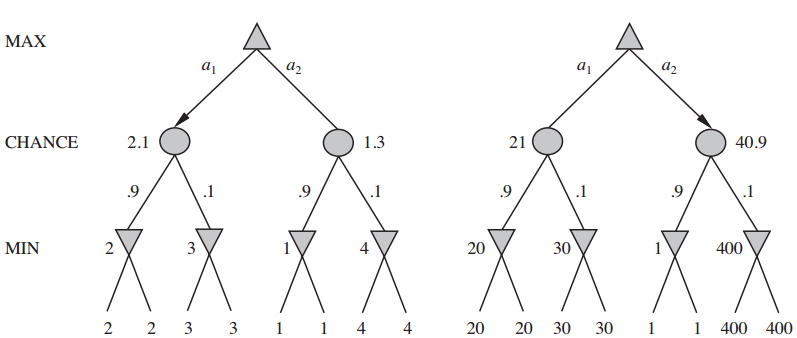
\includegraphics[width=1\textwidth]{expectimax-fig1.PNG}
      \caption{Os nodos de chance no jogo Catan, por exemplo, seriam as possibilidades ao jogar os dados.~\cite[Cap 5, pp177-180]{AIMA}}
    \end{figure}

%- Como esses elementos fogem do controle do agente, os valores de recompensa de minimax vistos anteriormente tem de ser substituidos por uma função de valor esperado, que leva em conta a média das possibilidades possíveis.

%---------------------------------------------------------------


\section{\label{sec:secao4}Tomada de Decisão em Ambientes Estocásticos}

\subsection{\label{sec:secao4.1}\textit{Markov Decision Process} (MDP)}

Um MDP busca encontrar a política que garanta a maior recompensa em um sistema de decisões sequenciais, observável e estocástico, definindo uma coleção de estados, ações, um modelo de transição e uma função de recompensa. Os estados representam diferentes situações do problema e as ações definem transições entre estados. O modelo de transição determina a probabilidade de se atingir um certo estado $x'$ se uma ação $a$ é aplicada à partir de um estado $x$. A função de recompensa define a utilidade de cada estado para o agente. A política é um mapeamento de estados para ações que define qual ação deve ser escolhida partindo de um determinado estado.
%bullet- Existe uma política ótima que resolve o problema com o melhor aproveitamento de utilidades.

Se o sistema de decisões for parcialmente observável, o problema se torna mais complexo. \textit{Partially Observable Markov Decision Processes} (POMDPs) é o nome da classe de problemas que possui essa característica. Como Catan é parcialmente observável devido as cartas de desenvolvimento e as trocas aleatórias de recursos entre jogadores, o agente não tem o modelo de transição e se encaixa nesta categoria.
Uma abordagem para resolver POMDPs é calcular a distribuição de probabilidade de todos os estados do problema com base nas decisões anteriores, e a partir deste cálculo, reduzir o problema em um MDP para esta distribuição.~\cite[Cap 17, pp645-647]{AIMA}

%bullet- Se o problema de Markov não tiver o modelo de transição disponível, o processo de se descobrir as utilidades passa a ser parte do %problema. \textit{Partially Observable Markov Decision Processes} (POMDPs) é o nome da classe de problemas que possui essa %caracteristica. Como Catan é estocástico e não observável, o agente não tem o modelo de transição e se encaixa nesta categoria.

%--------------------------------------------------------------

\subsection{\label{sec:secao4.2}Aprendizado por Reforço}

%\subsection{\label{sec:secao4.1}Recompensa}

%- Em um ambiente dinâmico como o de um jogo, a utilidade de uma ação em um determinado estado não é estática e depende de muitas variáveis.

%- É mais interessante para um agente em um ambiente como esse, buscar a melhor recompensa sempre que possível.

%- Logo, para descobrir recompensa de uma jogada, o agente deverá simular o jogo até o seu fim ou o mais próximo disso.

Aprendizado por Reforço é uma técnica de aprendizado onde um agente aprende o que fazer diante de um problema a partir de recompensas obtidas ao tentar resolvê-lo repetidas vezes, durante um treinamento ~\cite[Cap 21, pp830-859]{AIMA}. Recompensas, neste caso, são as mesmas vistas em MDPs, e o objetivo do agente ainda é encontrar uma política ótima para lidar com um problema. Em um jogo como Catan, as recompensas podem ser vistas como ganhar um ponto de vitória, vencer a partida ou perder a partida, o último seria um estimulo negativo para o agente.

Diferente de outros métodos de aprendizado, este não necessita de supervisão humana. Em aprendizado supervisionado, por exemplo, um humano informa ao agente qual é a ação correta a ser tomada a partir de um estado e o agente aprende com estas orientações ~\cite[Cap 18, pp695-697]{AIMA}. Por conta disso, aprendizado por reforço é mais adequado para jogos de tabuleiro, onde informar o agente sobre o que fazer para todos os estados de jogo pode ser impraticável. Sem informações prévias sobre todos os estados e resultados de ações, ou seja, o modelo de transição da MDP, o agente deve aprender a lidar com uma MDP desconhecida.

\subsection{\label{sec:secao4.3}Exploração e Lucro}

%Exploração e lucro são conceitos chave no aprendizado por reforço que também são importantes na construção de um agente capaz de aprender estratégias em jogos de tabuleiro. Um agente que visa aprender a melhor estratégia para certo jogo, precisa explorar o maior número de nodos da árvore de jogo o possível, afim de aprender quais nodos são mais lucrativos. O problema é que pode ser impossível para o agente explorar todas as possibilidades de jogadas da árvore de jogo e avaliar o resultado de todas as suas combinações em tempo hábil, ele deve decidir então quais e quantos serão os nodos que ele irá explorar desta árvore. O agente deve então decidir se prioriza o lucro imediato ou a exploração de novos estados. Priorizar o lucro imediato pode ser mais eficiente, mas uma jogada melhor pode estar escondida por traz de um estado não lucrativo, que o agente ainda não explorou. Encontrar o equilíbrio ideal entre explorar e lucrar se torna extremamente importante no processo de aprendizado do agente.

Exploração e lucro são conceitos chave no aprendizado por reforço ~\cite[Cap 21, pp830-859]{AIMA}. Visto que o agente deve aprender o modelo de transição sem ter conhecimento do modelo real do ambiente, se ele priorizar o lucro imediato, ele poderá estar aprendendo um modelo equivocado, que não representa o problema. Para que o agente aprenda o modelo de transição ótimo, ele deve também considerar ações pouco lucrativas a fim de conhecer mais sobre o modelo de transição real do ambiente.

O agente deve buscar então uma estratégia de exploração ótima. Essa estratégia deve explorar o problema para obter o máximo de aprendizado em um primeiro momento e depois passar para uma fase de lucro, explorando mais profundamente os nodos que geraram mais lucro, de modo que o modelo aprendido pelo agente seja ótimo com o menor esforço de exploração possível.

%Teoricamente, existe uma estratégia de exploração ótima, que prioriza a exploração até o ponto em que ela é útil e 

%bullet - Exploração e lucro são conceitos chave no aprendizado por reforço e são essenciais para resolver jogos.

%bullet - Durante o processo de busca pela jogada ótima, pode ser impraticavel para o agente explorar todas as possibilidades da arvore de jogo, e o agente deve decidir se prioriza o lucro imediato ou exploração.

%bullet - A jogada ótima pode estar "escondida" por uma jogada que parece ruim a curto prazo e por isso priorizar o lucro nem sempre leva até o melhor desempenho.

%bullet - Utilizando uma política de exploração, o agente pode explorar estados que parecem ruins mas na realidade são melhores do que estados de lucro conhecido.

%bullet- Encontrar uma política de exploração ótima não é trivial.

\subsection{\label{sec:secao4.4}Problema das N-Máquinas Caça-Níqueis}

O problema das N-máquinas caça-niqueis é estudado na área de decisões estatísticas e busca por uma política de exploração ótima ~\cite{BANDITSPROBLEMS}. Se encararmos problemas de decisão como a escolha de qual máquina caça-níquel paga mais dentre diversas máquinas independentes em um exato momento, podemos descobrir a melhor política de exploração dentre as máquinas de acordo com a a distribuição de lucros observada depois de investir em todas as máquinas repetidas vezes. Pode não ser possível investir em todas as máquinas o número de vezes necessário para se descobrir a melhor política, mas é possível garantir uma política que converge para a política ótima conforme o número de investimentos sobe, e pode-se chegar em uma aproximação satisfatória dentro do limite de simulação disponível.

%O arrependimento é um conceito importante para os métodos que se baseiam no problema das máquinas caça-níqueis para encontrar a política de exploração ótima.~\cite{Monte-CarloSurvey} Ele representa quanto o agente investiu nas máquinas até aprender a melhor estratégia e é definido, após $\mathit{n}$ jogadas.

%\begin{equation*}
%\mathit{R_{N}} = \mu^\star\mathit{n}- {\mu_{j}}\sum\limits_{j=1}^K \mathbb{E}[\mathrm{T_{j}}\mathit{(n)}]
%\end{equation*}

%Onde $\mu^\star$ é a melhor recompensa possível e $\mathbb{E}[\mathrm{T_{j}}\mathit{(n)}]$ representa o número de vezes em que se investiu em uma máquina $_{j}$ dentro destas $\mathit{n}$ jogadas.

%Devemos minimizar ao máximo o arrependimento para garantir a melhor performance do agente e evitar disperdício de recursos durante a exploração. Sabemos que o arrependimento nunca cresce menos do que $\mathcal{O}(\ln{}n)$ durante o processo de exploração ~\cite{regretBandits}, e assim, podemos concluir que temos um equilíbrio perfeito entre exploração e lucro quando o arrependimento cresce em um fator constante de $\mathcal{O}(\ln{}n)$.

%\subsection{\label{sec:secao4.3}\textit{Upper-Confidence-Bound}(UCB)}

%Para essa classe de problemas, é útil sabermos qual é o intervalo de confiança superior, {Upper-Confidence-Bound} (UCB), que qualquer máquina será ótima. Existe uma política de UCB que possui um crescimento logaritmico e não necessita de nenhum conhecimento prévio da distribuição de recompensas entre as máquinas, chamado UCB1. ~\cite{refUCB} Podemos então utilizar essa política UCB1 para ajudar na escolha de qual máquina investir buscando esse equilíbrio entre exploração e lucro.

%*IREMOS COLOCAR AQUI A FUNÇÃO DA UCB1*

\subsection{\label{sec:secao4.5}\textit{Q-Learning}}

Dentre as técnicas de aprendizado por reforço, \textit{Q-Learning} se diferencia das outras por ser uma técnica livre de modelo de transição ~\cite{QLEARNING}. Em \textit{Q-Learning} o agente aprende um valor de recompensa associado à uma tupla ação-estado que converge para resultados similares ao de se aprender o modelo de transição, o que significa que o agente necessita de menos conhecimento do domínio, simplificando o processo de aprendizado, porém restringindo o seu potencial de aprender em ambientes complexos, já que ele não poderá simular os resultados das ações possíveis. Enquanto outras técnicas visam aprender o modelo de transição da MDP desconhecida, esta técnica não necessita do modelo para aprender a resolver o problema.

%\textit{Q-Learning} funciona com uma variável Q, ou \textit{Q-Value}. O \textit{Q-Value} é o valor da recompensa associado à uma tupla ação-estado. Essa variável é análoga a informação de utilidade de uma MDP. Utilizando esta técnica, o agente aprende o \textit{Q-Value} dos estados explorados e utiliza essa informação para decidir sua ação.

%---------------------------------------------------------------------------------------------------

%\section{\label{sec:secao5}Métodos de Monte-Carlo}

\section{\label{sec:secao5}\textit{Monte-Carlo Tree Search} (MCTS)}

\textit{Monte-Carlo Tree Search} é uma família algoritmos modernos para resolver problemas, principalmente jogos, que não exige conhecimento do domínio do problema para obter resultados satisfatórios ~\cite{MONTECARLOSURVEY}. Uma vantagem desse algoritmo em relação ao Minimax é que ele pode ser usado em jogos estocásticos e parcialmente observáveis, enquanto o Minimax necessita de adaptações para cumprir tais requisitos. 

    \begin{figure}[H]
      \centering
      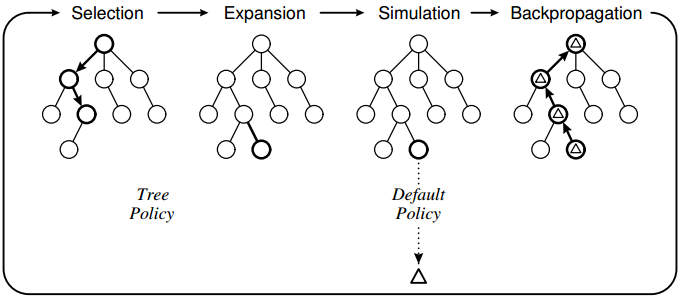
\includegraphics[width=1\textwidth]{EieiQ.png}
      \caption{Etapas da Àrvore de Pesquisa de Monte-Carlo}
    \end{figure}


O algoritmo funciona em 4 estágios, de acordo com a Figura 2.5. A partir de um nodo raiz, o algoritmo expande os próximos nodos possíveis. Cada nodo possui uma informação estatística que ajuda o algoritmo a decidir qual será o próximo nodo a ser explorado. Seguem as descrições de cada estágio do algoritmo:

\begin{itemize}

   \item Seleção: Do nodo raiz, é selecionado um nodo inexplorado da árvore de jogo a partir de uma politica de seleção, que escolhe a jogada mais promissora buscando lucrar ou explorar.
   
   \item Expansão: Um ou mais nodos são adicionados como filhos do nodo selecionado a partir das jogadas válidas possíveis.
   
   \item Simulação: O jogo é simulado a partir de um ou mais nodos gerados na fase de expansão seguindo uma política de jogo padrão, que pode ser movimentos aleatórios, semi-aleatórios ou algo mais sofisticado. Quanto mais sofisticada a política padrão, mais custosa e lenta será a simulação.
   
   \item Propagação Inversa: Com a recompensa obtida na fase de Simulação, a informação estatística de cada nodo é atualizada, partindo do nodo adicionado até a raiz.
   
\end{itemize}

Com uma quantidade suficiente de simulações, a melhor jogada pode ser inferida a partir de uma política de jogo padrão simples, ou até mesmo aleatória, devido a experiência obtida pela propagação dos resultados da simulação na árvore ~\cite{MONTECARLOSURVEY}. Uma função de exploração é essencial para os algoritmos de Monte-Carlo e dentre os mais populares e efetivos, estão os métodos que se baseiam no problema das N-máquinas caça-niquel.


%- Cada nodo guarda 2 valores que compoem as suas informações estatisticas:

%\begin{itemize}

   %\item \textit{Q-Value}: O valor de recompensa que foi obtido escolhendo tal nodo. Equivalente ao usado em \textit{Q-Learning}.
   
   %\item Numero de Visitações: Quantas vezes este nodo já foi escolhido para ser explorado.
   
%\end{itemize}

Uma MCTS pode ser vista como um tipo de aprendizado por reforço ~\cite{MONTECARLOSURVEY}. Ambas as técnicas utilizam uma amostragem de simulações para construir conhecimento acerca do problema. Sob certas circunstâncias, ambos os algoritmos podem até ser equivalentes ~\cite{MONTECARLOREINFORCEMENTEQ}, mas algoritmos de aprendizado por reforço, como \textit{Q-Learning}, geralmente não constroem árvores. Outra diferença é que para decidir qual será a próxima ação, MCTS estima valores temporários para cada estado, enquanto aprendizado por reforço, como \textit{Q-Learning}, estima valores a longo prazo, que então ajudarão o agente a tomar decisões futuras ~\cite{MONTECARLOSURVEY}.

%\subsection{\label{sec:secao5.2}\textit{Upper Confidence Bounds for Trees} (UCT)}

%\subsection{\label{sec:secao5.3}Variações de MCTS}

%Existem muitas variações do algoritmo básico de MCTS visando diferentes tipos de problemas, vamos abordar aqui algumas das mais significativas para o nosso trabalho.

%-----------------------------------------------------------------

%----------------------------------------------------------------------------------


%OBJETIVOS
%----------------------------------------------------------------------------------

\chapter{\label{chap:objetivos}Objetivos}

Este trabalho tem como objetivo desenvolver uma IA capaz de jogar o jogo Colonizadores de Catan e medir a sua capacidade de jogo.

%-----------------------------------------------------------------
\section{\label{sec:gerais}Objetivo Geral}

Projetar uma IA capaz de jogar Colonizadores de Catan, utilizando o conhecimento adquirido no estudo do cliente do jogo e das técnicas de IA descritas nesta proposta.

%-----------------------------------------------------------------

%-----------------------------------------------------------------
\section{\label{sec:espec}Objetivos Específicos}

    \begin{itemize}

        \item Compreender e modelar formalmente o jogo Colonizadores de Catan, com o estudo do cliente de jogo \textit{JSettlers}.

        \item Entender algoritmos clássicos baseados no Minimax.

        \item Compreender como os algoritmos de Aprendizado por Reforço podem ajudar o agente a aprender as regras de jogo e sua relação com MCTS.

        \item Entender o funcionamento de técnicas de MCTS e escolher aquelas que serão importantes no Colonizadores de Catan.
        
        \item Descobrir outras técnicas de IA capazes de melhorar a performance de um agente no jogo.

        \item Implementar um pequeno protótipo para um ou mais algoritmos de IA descritos nesta proposta.

        \item Projetar um agente capaz de jogar Colonizadores de Catan utilizando um ou mais dos algoritmos estudados.
    
    \end{itemize}

%-----------------------------------------------------------------

%----------------------------------------------------------------------------------


%ANALISE E PROJETO
%----------------------------------------------------------------------------------

\chapter{\label{chap:ana&proj}Análise e Projeto}

Afim de atingir os objetivos, será necessário a realização de algumas atividades como, entender as estratégias do jogo Colonizadores de Catan e técnicas de IA que podem ser aplicadas para resolve-lo. O detalhamento destas atividades será visto a seguir.

%-----------------------------------------------------------------
\section{\label{sec:ativ}Atividades}

    \begin{itemize}

        \item Estudar o cliente \textit{JSettlers}: O cliente \textit{JSettlers} é uma implementação em Java do jogo Colonizadores de Catan. O estudo irá contribuir para a implementação da IA que irá jogar neste cliente.
   
        \item Estudar o algoritmo Minimax: O Minimax é um algoritmo voltado para IA em jogos. Seu funcionamento, aplicando algumas técnicas, pode ser aproveitado na realização da IA que joga Catan.
   
        \item Estudar tomada de decisão: Há diversos algoritmos que buscam encontrar a política ótima em um sistema de decisões sequenciais, fazendo assim o agente realizar uma ação apropriada para o momento. Fundamental para o entendimento dos algoritmos estudados.
   
        \item Estudar aprendizado por reforço: O aprendizado por reforço utiliza a noção de recompensas para ensinar agentes como se comportar diante de um problema. Esta abordagem pode ser aproveitada como uma alternativa para o agente aprender sobre o jogo proposto.
        
        \item Estudar \textit{Monte-Carlo Tree Search}: Este é um algoritmo moderno que teve muito sucesso quando aplicado a diversos jogos. Ele utiliza uma amostragem de simulações para construir conhecimento acerca de um problema. O estudo de técnicas baseadas neste algoritmo podem contribuir na criação da IA que jogará Catan.
        
        \item Pesquisar outras técnicas: Estudaremos também outras técnicas que podem ser utilizadas para melhorar a performance da IA.
            
        \item Modelagem do agente: Será realizada a modelagem de um agente capaz de jogar o jogo no cliente \textit{JSettlers} que possa utilizar mais de uma das técnicas estudadas.
        %\item Implementar o protótipo: O protótipo será realizado para experimentar algumas das técnicas de IA apresentadas.
   
    \end{itemize}

%-----------------------------------------------------------------

%-----------------------------------------------------------------
\section{\label{sec:crono}Cronograma}

    \begin{figure}[H]
      \centering
      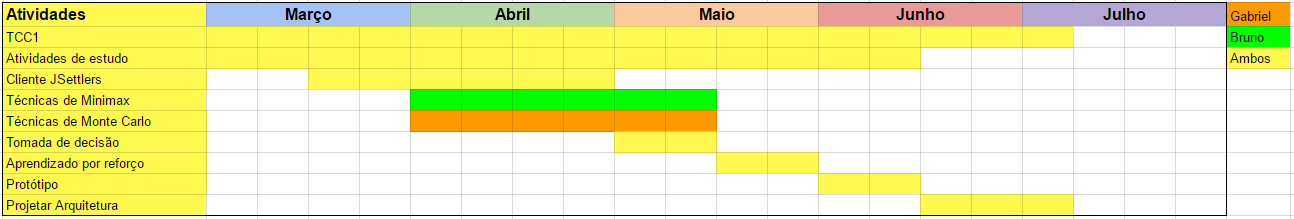
\includegraphics[width=1\textwidth]{crono.PNG}
      \caption{Cronograma das atividades planejadas.}
    \end{figure}
%-----------------------------------------------------------------

%----------------------------------------------------------------------------------

%----------------------------------------------------------------
% Aqui vai a bibliografia. Existem 3 estilos de citação: use
% 'tcc-alpha' para citações do tipo [Abc+] ou [XYZ] (em ordem
% alfabética na bibliografia), 'tcc-num' para citações
% numéricas do tipo [1], [20], etc., em ordem de referência e
% 'tcc-alpha-full' para citações estilo 'alpha' mas com nomes completos.
%----------------------------------------------------------------
\bibliographystyle{tcc-alpha}
%\bibliographystyle{tcc-num}
\bibliography{exemplo-bib}

% E aqui (para a felicidade de todos) termina o documento.
\end{document}